\label{sec:results-lcft}
We explore \model's ability to work with long sequences by measuring perplexity, key retrieval accuracy and performance during generation on code completion tasks. These tasks, and our results are detailed below. 
For full results and comparisons to alternative techniques of increasing the context length of LLMs, we refer to~\Cref{app:lcft}.

\paragraph{Perplexity during extrapolation.} In \Cref{fig:lcft-code-ppl}, perplexity is computed over 4M tokens from the code dataset, using a subset of our validation data consisting of large source files ($\ge$50kB).
For all model sizes, we observe a steady decrease in perplexity well beyond 16384 tokens, which is the sequence length we use for long-context fine-tuning.
After 100K tokens, the perplexity increases only slightly, in contrast to the well-known instability phenomenon when testing transformer models on sequences larger than those seen during training~\citep{press2021train}.

\paragraph{Key retrieval.} In \Cref{fig:lcft-key-retrieval}, we investigate key retrieval performance in synthetic task.
The prompt consists of a large amount of syntactically valid Python code, with a function returning a scalar inserted at a specified position.
The model is asked to complete an \texttt{assert} statement with the return value of the inserted function.
\citet{liu2023lost} showed that the inability to recall content placed in the middle of long prompts is a common failure mode in LLMs; our retrieval task is analogous to their setup, albeit tailored to code models which are not fine-tuned to follow instructions. 
All models exhibit strong retrieval performance on the sequence length they were trained on, with the exception of the 7B model for test cases in which the function is placed at the beginning of the prompt.
We include OpenAI’s gpt-3.5-turbo-16k-0613 as a reference. We query GPT with a system prompt of ``Complete the following code.'' and a temperature of 0. 
For sequences beyond 16K tokens, i.e., when extrapolating, our models exhibit a decrease in performance (\Cref{app:lcft_extended_results}).

\begin{figure}[t!]
     \centering
     \begin{subfigure}[T]{0.45\textwidth}
         \centering
         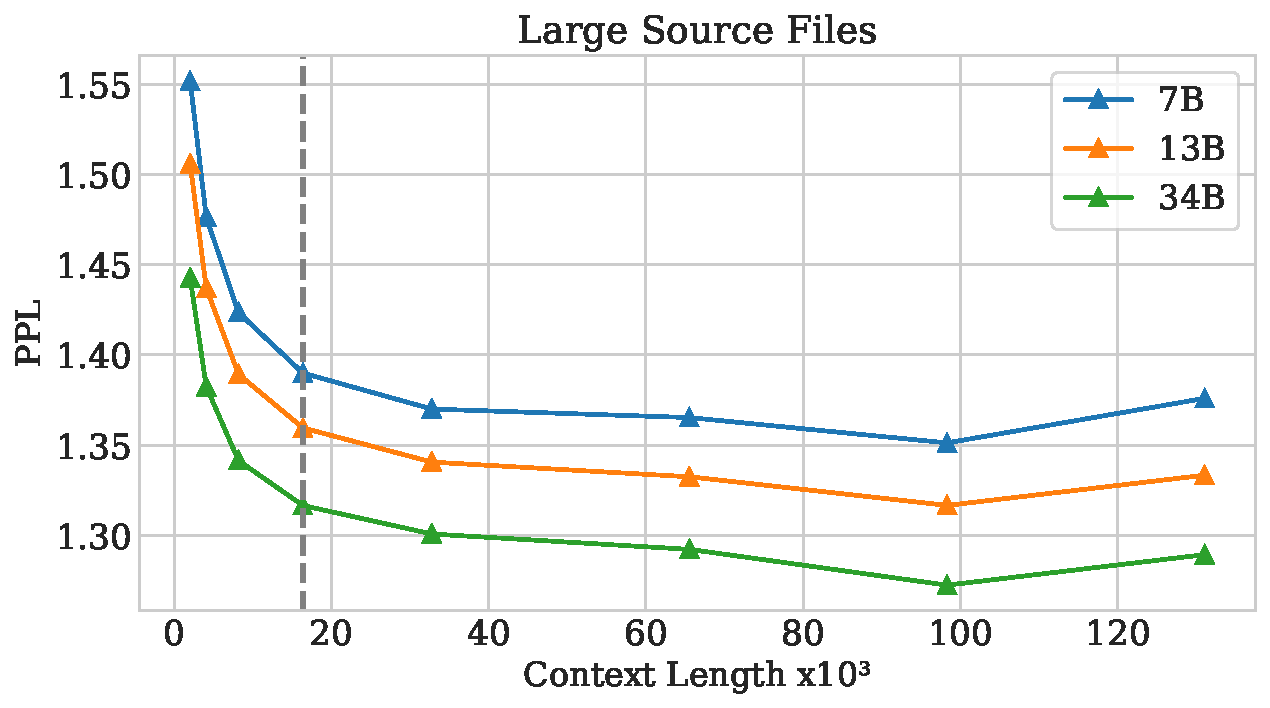
\includegraphics[width=\textwidth]{figs/code_long_valid_ppl.pdf}
         \caption{}
         \label{fig:lcft-code-ppl}
     \end{subfigure}
     \hfill
     \begin{subfigure}[T]{0.45\textwidth}
         \centering
         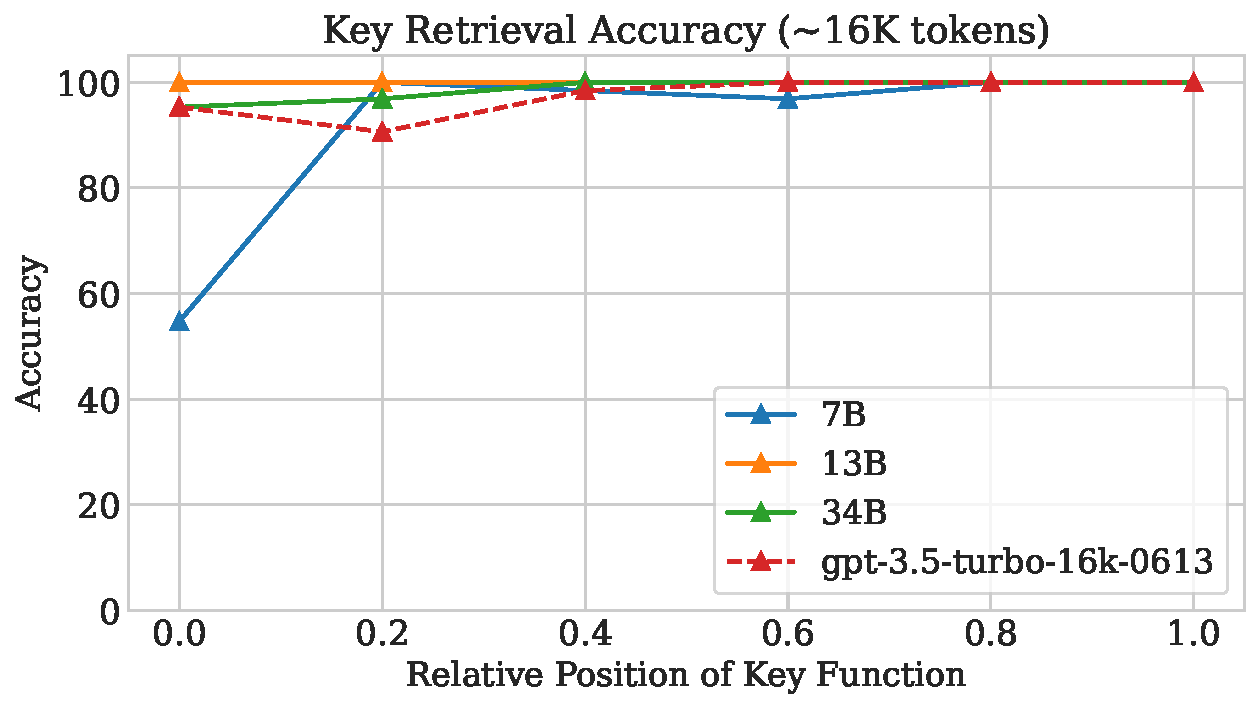
\includegraphics[width=\textwidth]{figs/function_key_retrieval.pdf}
         \caption{}
         \label{fig:lcft-key-retrieval}
     \end{subfigure} \\
    \caption{\textbf{\model behavior on long sequences.}
    \textbf{(a)} Perplexity on large source files ($\ge$50 kB) from the validation data from the code dataset. The dashed line marks the fine-tuning context length. Perplexity decreases for up to 100K tokens for all \model sizes.
    \textbf{(b)} Accuracy on a synthetic key retrieval task, with a context of 16K tokens and comparison to gpt-3.5-turbo.
    }
    \label{fig:long_sequences}
\end{figure}


\paragraph{Single line completion.} Finally, we test the benefits of the ability to handle long context sizes in a single line code completion task.
Our task is based on the Long Code Completion (LCC) benchmark~\citep{guo2023longcoder}.\footnote{Note that LCC data points are included in our code training data.}
The LCC test set is skewed towards shorter files and we hence sample a new set of examples from LCC's validation and test set with an equalized distribution over file size (\Cref{app:lcft_benchmarks}).
In \Cref{tab:lcc_results}, we compare the completion accuracy of the \model models to their counterparts prior to long-context fine-tuning.
Non-LCFT models fail to generate meaningful completions on long sequences and we thus truncate their prompts to the 4,000 tokens immediate preceding the line to complete.
Across all metrics, models fine-tuned to handle long contexts achieve significantly higher performance.
This demonstrates that long contexts are informative for code completion, and that with LCFT our models are able to leverage this information to improve their generations. 
We note that the longest example's prompt in this test consists of 103K tokens, for which all \model models generate syntactically correct completions, with the 7B model producing an exact match.

\paragraph{Performance impact on short contexts.}
While our models are effective on long sequences, we observe that LCFT slightly hurts performance on standard code synthesis benchmarks consisting of short sequences.
In \Cref{tab:full_res}, we observe an average decrease of 0.52 percentage points on HumanEval pass@1 and 1.9 points on MBPP for the pass@1 metric.
Similarly, a breakdown of the code completion results in \Cref{tab:lcc_results} by the number of tokens in each example shows that for prompts shorter than 4k tokens, long context fine-tuning induces a reduction of up to 2 BLEU points from base models after code training (\Cref{fig:lcft-lcc-difference}).
We observe similar decreases in performance for infilling tasks (Table~\ref{tab:he-fim-incoder}).

LCFT comes at a cost for short sequences, and slightly decreases our scores on standard coding benchmarks such as HumanEval and MBPP. However, many real-world use cases are not captured by these benchmarks, and we believe that this cost is more than offset by the potential of handling long sequences for real downstream applications. Hence we opt to release all our \model, \pymodel and \instmodel models with long-context capabilities.


\begin{table}[]
\centering
\begin{tabular}{lcccccccc}
\toprule
Model &   \\
& & & EM & BLEU & EM & BLEU & EM & BLEU \\
\midrule
\model & 7B & \ding{55} & 36.86 & 60.16 & 47.82 & 69.20 & 46.29 & 67.75 \\
\model & 7B & \ding{51} & \textbf{39.23} & \textbf{61.84} & \textbf{51.94} & \textbf{71.89} & \textbf{50.20} & \textbf{70.22} \\
\midrule
\model & 13B & \ding{55} & 37.96 & 61.33 & 50.49 & 69.99 & 49.22 & 69.87 \\
\model & 13B & \ding{51} & \textbf{41.06} & \textbf{62.76} & \textbf{52.67} & \textbf{72.29} & \textbf{52.15} & \textbf{71.00} \\
\midrule
\model & 34B & \ding{55} & 42.52 & 63.74 & 54.13 & 72.38 & 52.34 & 71.36 \\
\model & 34B & \ding{51} & \textbf{44.89} & \textbf{65.99} & \textbf{56.80} & \textbf{73.79} & \textbf{53.71} & \textbf{72.69} \\
\bottomrule
\end{tabular}%
%}
\caption{\textbf{Average single line completion performance on LCC-balanced.} Comparison of models before and after long-context fine-tuning in terms of exact match (EM) and BLEU.
For non-LCFT models, context size limits are respected by truncating prompts to 4,000 tokens.
}
\label{tab:lcc_results}
\end{table}
